% Options for packages loaded elsewhere
\PassOptionsToPackage{unicode}{hyperref}
\PassOptionsToPackage{hyphens}{url}
\PassOptionsToPackage{dvipsnames,svgnames,x11names}{xcolor}
%
\documentclass[
  10pt,
]{article}
\usepackage{amsmath,amssymb}
\usepackage{iftex}
\ifPDFTeX
  \usepackage[T1]{fontenc}
  \usepackage[utf8]{inputenc}
  \usepackage{textcomp} % provide euro and other symbols
\else % if luatex or xetex
  \usepackage{unicode-math} % this also loads fontspec
  \defaultfontfeatures{Scale=MatchLowercase}
  \defaultfontfeatures[\rmfamily]{Ligatures=TeX,Scale=1}
\fi
\usepackage{lmodern}
\ifPDFTeX\else
  % xetex/luatex font selection
  \setmainfont[]{DejaVu Serif}
  \setmonofont[]{DejaVu Sans Mono}
\fi
% Use upquote if available, for straight quotes in verbatim environments
\IfFileExists{upquote.sty}{\usepackage{upquote}}{}
\IfFileExists{microtype.sty}{% use microtype if available
  \usepackage[]{microtype}
  \UseMicrotypeSet[protrusion]{basicmath} % disable protrusion for tt fonts
}{}
\makeatletter
\@ifundefined{KOMAClassName}{% if non-KOMA class
  \IfFileExists{parskip.sty}{%
    \usepackage{parskip}
  }{% else
    \setlength{\parindent}{0pt}
    \setlength{\parskip}{6pt plus 2pt minus 1pt}}
}{% if KOMA class
  \KOMAoptions{parskip=half}}
\makeatother
\usepackage{xcolor}
\usepackage[margin=18mm]{geometry}
\usepackage{longtable,booktabs,array}
\usepackage{calc} % for calculating minipage widths
% Correct order of tables after \paragraph or \subparagraph
\usepackage{etoolbox}
\makeatletter
\patchcmd\longtable{\par}{\if@noskipsec\mbox{}\fi\par}{}{}
\makeatother
% Allow footnotes in longtable head/foot
\IfFileExists{footnotehyper.sty}{\usepackage{footnotehyper}}{\usepackage{footnote}}
\makesavenoteenv{longtable}
\usepackage{graphicx}
\makeatletter
\def\maxwidth{\ifdim\Gin@nat@width>\linewidth\linewidth\else\Gin@nat@width\fi}
\def\maxheight{\ifdim\Gin@nat@height>\textheight\textheight\else\Gin@nat@height\fi}
\makeatother
% Scale images if necessary, so that they will not overflow the page
% margins by default, and it is still possible to overwrite the defaults
% using explicit options in \includegraphics[width, height, ...]{}
\setkeys{Gin}{width=\maxwidth,height=\maxheight,keepaspectratio}
% Set default figure placement to htbp
\makeatletter
\def\fps@figure{htbp}
\makeatother
\setlength{\emergencystretch}{3em} % prevent overfull lines
\providecommand{\tightlist}{%
  \setlength{\itemsep}{0pt}\setlength{\parskip}{0pt}}
\setcounter{secnumdepth}{-\maxdimen} % remove section numbering
\ifLuaTeX
  \usepackage{selnolig}  % disable illegal ligatures
\fi
\usepackage{bookmark}
\IfFileExists{xurl.sty}{\usepackage{xurl}}{} % add URL line breaks if available
\urlstyle{same}
\hypersetup{
  colorlinks=true,
  linkcolor={Maroon},
  filecolor={Maroon},
  citecolor={Blue},
  urlcolor={Blue},
  pdfcreator={LaTeX via pandoc}}

\author{}
\date{}

\begin{document}

\section{Exact symmetry of the eight twist-derived
kernels}\label{exact-symmetry-of-the-eight-twist-derived-kernels}

On the fixed public p827 example, the certified degree17 endomorphism
cycles through all48 nonzero twist seven-torsion points and all eight
kernel lines. Native computation and independent PARI/GP agree. These
are exact finite computations, not measured relation-solving costs.

\begin{longtable}[]{@{}
  >{\raggedright\arraybackslash}p{(\columnwidth - 6\tabcolsep) * \real{0.2500}}
  >{\raggedleft\arraybackslash}p{(\columnwidth - 6\tabcolsep) * \real{0.2500}}
  >{\raggedleft\arraybackslash}p{(\columnwidth - 6\tabcolsep) * \real{0.2500}}
  >{\raggedleft\arraybackslash}p{(\columnwidth - 6\tabcolsep) * \real{0.2500}}@{}}
\toprule\noalign{}
\begin{minipage}[b]{\linewidth}\raggedright
Recorded quantity
\end{minipage} & \begin{minipage}[b]{\linewidth}\raggedleft
Actual action
\end{minipage} & \begin{minipage}[b]{\linewidth}\raggedleft
Identity control
\end{minipage} & \begin{minipage}[b]{\linewidth}\raggedleft
Scalar2 control
\end{minipage} \\
\midrule\noalign{}
\endhead
\bottomrule\noalign{}
\endlastfoot
Point order & 48 & 1 & 3 \\
Projective order & 8 & 1 & 1 \\
Direct point checks & 49 & --- & --- \\
Addition checks & 2401 & --- & --- \\
Direct kernel-root matches & 8 & --- & --- \\
\end{longtable}

\begin{figure}
\centering
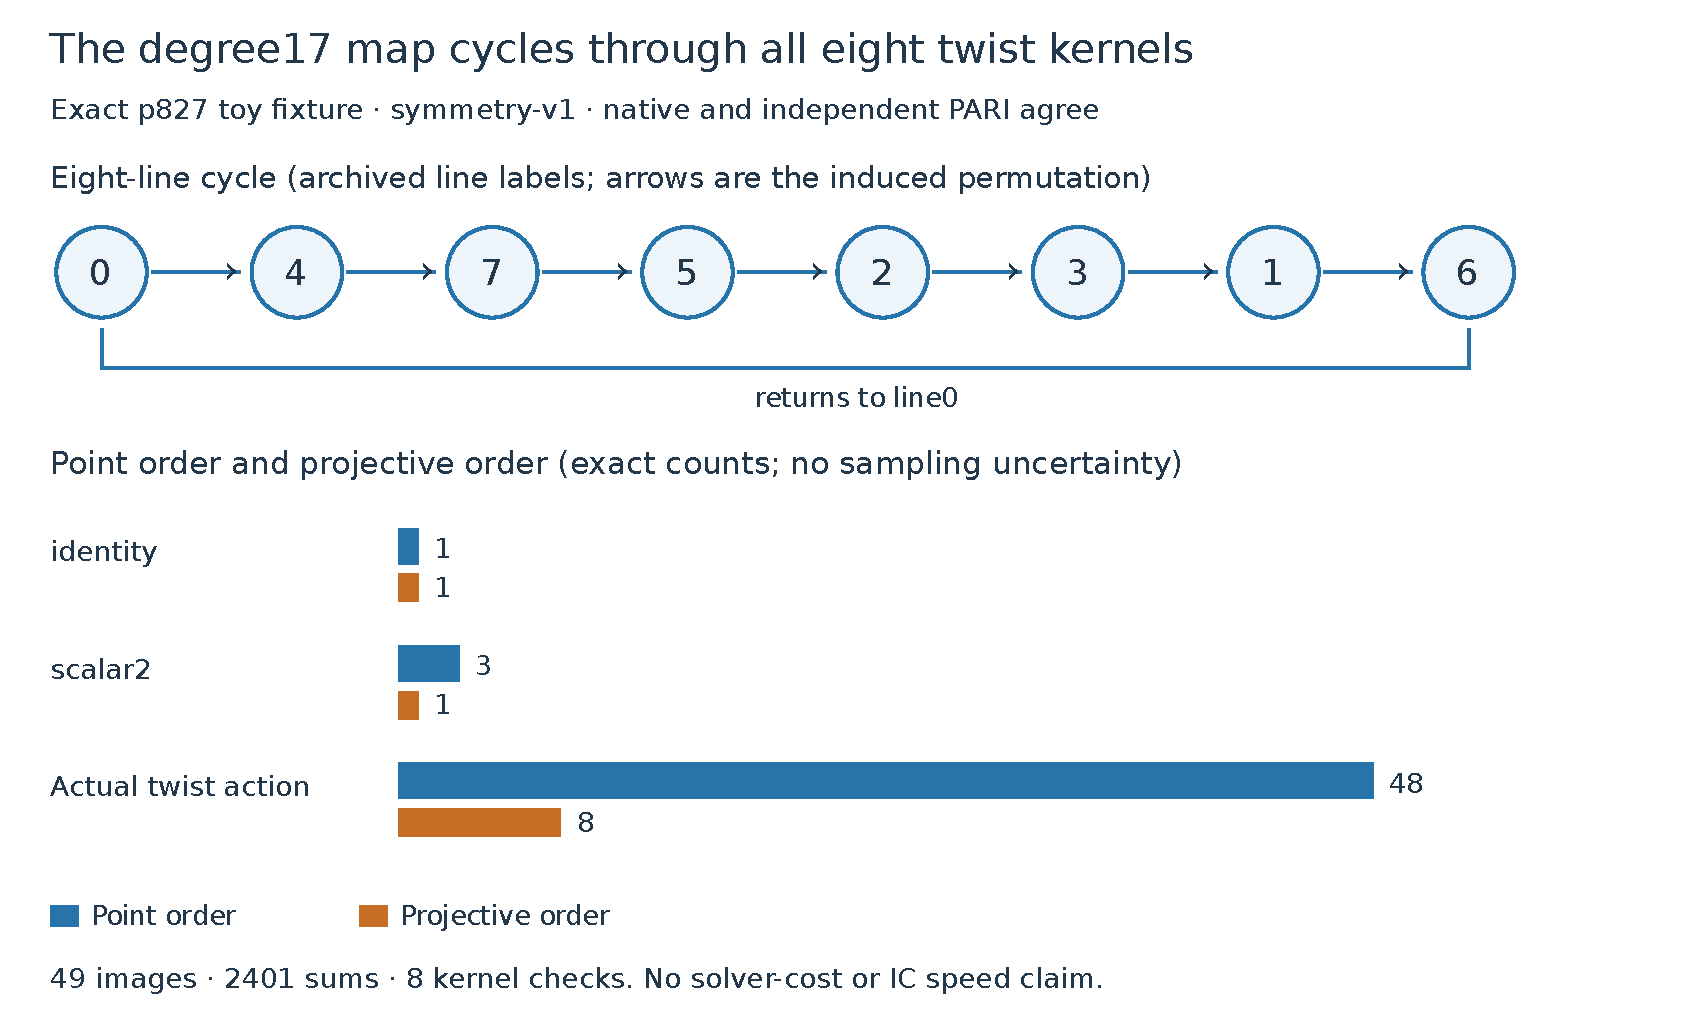
\includegraphics{SYMMETRY.pdf}
\caption{Recorded cycle and exact orders; run symmetry-v1. Complete
finite populations, no statistical uncertainty.}
\end{figure}

The source is \(E:y^2=x^3+x+15\) over \(\mathbb F_{827}\), ICV1
\texttt{icv1-fp10-t5-192cb216}, order823, generator(2,5). Its quadratic
twist \(T:Y^2=X^3+4X+120\) has order833. The unchanged archived basis of
\(T[7]\) is \(T_1=(0,51)\) and \(T_2=(6,130)\); labels\((i,j)\) mean
\(iT_1+jT_2\). The endomorphism is the previously certified
\(\alpha=(\pi+[1])/[7]\).

In that basis its independently recovered matrix and eighth power are

\[M=\begin{pmatrix}3&1\\5&5\end{pmatrix}\pmod7,
\qquad M^2-M+3I=0,\qquad M^8=3I.\]

The complete nonzero point set is one48-cycle. Kernel labels are
\(\langle T_1+cT_2\rangle\) for \(c=0,\ldots,6\), followed by
\(\langle T_2\rangle\) as line7. Their single cycle is
\(0\to4\to7\to5\to2\to3\to1\to6\to0\). Every image line was checked by
matching its three paired kernel x-coordinates against the archived v8
kernel polynomial roots.

\subsection{Method, proof and scope}\label{method-proof-and-scope}

Native evaluation embeds into \(E(\mathbb F_{827^2})\), applies the
frozen normalized degree17 Vélu map and inverse-scale7 isomorphism, then
unembeds. GP independently reconstructs Vélu with \texttt{ellisogeny}
and evaluates the rational twist map \((X,Y)\mapsto(2R(X/2),Y S(X/2))\).
Each implementation reconstructs the matrix from point labels and checks
every point, all2401 additions, complete point/line cycles, trace1 and
determinant3. A corrupted coefficient is detected on42/49 points;
swapping two line images yields2/8 mismatches.

The proof is finite: a cyclic basis \((v,Mv)\) conjugates the matrix to
\(C=\left(\begin{smallmatrix}0&4\\1&1\end{smallmatrix}\right)\)
over\(\mathbb F_7\). Exhaustion establishes \(C^8=3I\), \(C^{48}=I\), no
shorter positive point period for any nonzero vector, and no shorter
positive line period than8. The full raw orbit, point and kernel records
are retained.

Four Lean declarations in \texttt{lean-v7/TwistKernelSymmetry.lean}
prove these companion-module statements by kernel-checked finite
arithmetic:

\begin{itemize}
\tightlist
\item
  \texttt{eighth\_scalar}: eighth power is scalar3.
\item
  \texttt{forty\_eighth\_identity}: forty-eighth power is the identity.
\item
  \texttt{nonzero\_point\_period}: every nonzero point has period48.
\item
  \texttt{projective\_period}: every nonzero line has period8.
\end{itemize}

Pinned Lean4.34.1/mathlib revision
\texttt{d13f23b7\allowbreak{}23b8a846\allowbreak{}827a245b\allowbreak{}89c10fc7\allowbreak{}d3f11612}; frozen replay and
fresh native transitive axiom audit pass with standard foundations only,
no trusted \texttt{native\_decide}. The concrete
elliptic-curve/torsion-basis/map-to-matrix bridge remains unformalized.
The v1 identity-certificate format fixes a different prime modulus and
cannot certify this characteristic7 action; the exact native/GP and Lean
evidence are the applicable certificates.

This supplies a finite symmetry relating all eight kernels. Induced
explicit maps between their quotient curves and any saving in
constructing or solving relations remain unmeasured. The point order48
on\(T[7]\) differs from the known scalar action's order274
on\(E(\mathbb F_{827})\). No degree1 automorphism, cheap rho fold,
novelty, full-IC improvement or NIST applicability is inferred.

\subsection{Reproducibility and
execution}\label{reproducibility-and-execution}

Source revision \texttt{ee305333\allowbreak{}dfb7c7ac\allowbreak{}c1916979\allowbreak{}4de12e6c\allowbreak{}6538a3be};
frozen protocol hash
\texttt{49ac79e2\allowbreak{}8023c2e4\allowbreak{}a23f27e2\allowbreak{}99419b8c\allowbreak{}b15ac577\allowbreak{}ba50a531\allowbreak{}ad43d6e0\allowbreak{}a2ac07dd}.
The frozen record was committed and Setec gate passed before data.
Native and GP each completed their single300s-capped run on the managed
Xeon8573C KVM host, one thread/CPU0/4GiB, L0; no clocks are admitted.

Flow: planned2, attempted2, completed2, not completed0, interrupted0,
resumed0, excluded0. Both strict admissions pass. Unified export binds
protocol, source, script, inputs and actual raw files with zero
findings. Independent implementation shares author/host; no
separate-runner review exists.

Raw archive is5432bytes/eight files, SHA256
\texttt{1f0992c7\allowbreak{}7000041a\allowbreak{}0d7d2be6\allowbreak{}d8642b5d\allowbreak{}5e161444\allowbreak{}2b3d07ab\allowbreak{}c4d7bd22\allowbreak{}c51e36d5},
in the user-confirmed \texttt{s3://setec-astronomy-artifacts/store}. See
execution-v11 for member inventory, deterministic recipe, fresh remote
verification and all exact commands. Synthetic native tests pass18/18;
all standalone runner tests pass. The prior full-root-suite validation
gap remains open separately.

Preserved development issues: missing finite-product Lean import was
fixed; draft placeholders/short SHA were rejected before freeze; the
initial export omitted host memory metadata and was retained, then
corrected with no science changes. Fresh ECR readiness remains
access-denied, so the documented authorized local fallback applies. No
paid resources or permissions were changed.

Literature: Andrew Sutherland, MIT18.783 Fall2025
\href{https://math.mit.edu/classes/18.783/2025/LectureNotes5.pdf}{Lecture5}
Theorems5.11/5.15,
\href{https://math.mit.edu/classes/18.783/2025/LectureNotes13.pdf}{Lecture13}
Theorems13.6/13.8, accessed/read2026-10-28; repository
\texttt{RESEARCH\_ISOGENY\_LOOP\_GLV.md} and atlas GLV/isogeny-loop
lead. These support the standard construction and distinction from
unknown-log recovery.

Canonical progress/IC/curve graphs were checked: this exact module
census does not change a performance row, model identity or previously
verified edge. Prior graphs and frozen waves remain unchanged.

\end{document}
